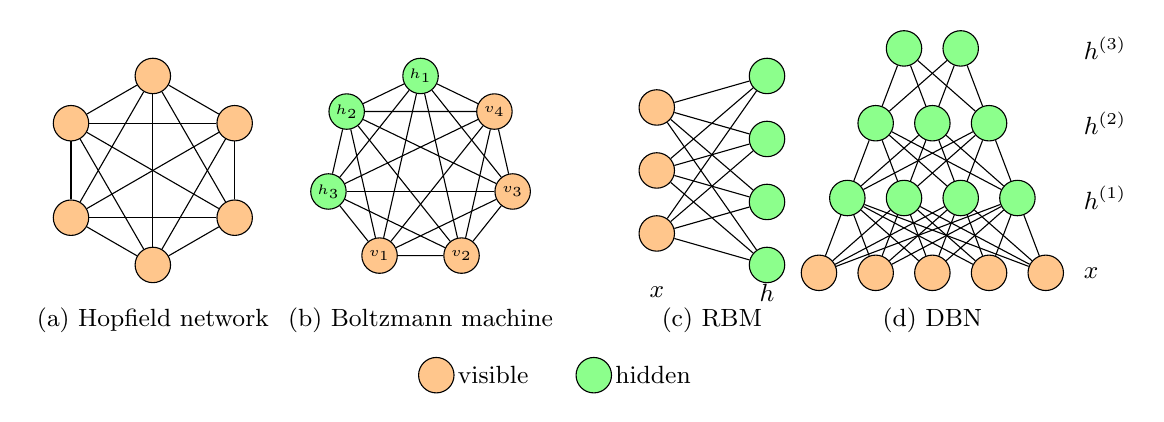
\begin{tikzpicture}[font=\small,
  vis/.style={circle, draw, fill=orange, fill opacity=0.45, text opacity=1, minimum size=4.5mm, inner sep=0pt},
  hid/.style={circle, draw, fill=green, fill opacity=0.45, text opacity=1, minimum size=4.5mm, inner sep=0pt}]
  % (a) Hopfield network: all units visible, complete graph
  \begin{scope}
    \foreach \k in {0,...,5} \node[vis] (a\k) at ({90+60*\k}:1.2) {};
    \foreach \i in {0,...,5} \foreach \j in {0,...,5} { \ifnum\i<\j \draw (a\i) -- (a\j); \fi }
    \node at (0,-1.9) {(a) Hopfield network};
  \end{scope}
  % (b) Boltzmann machine: visible and hidden units, complete graph
  \begin{scope}[xshift=3.4cm]
    \foreach \k/\t/\l in {0/hid/h_1,1/hid/h_2,2/hid/h_3,3/vis/v_1,4/vis/v_2,5/vis/v_3,6/vis/v_4}
      \node[\t, font=\tiny] (b\k) at ({90+360/7*\k}:1.2) {$\l$};
    \foreach \i in {0,...,6} \foreach \j in {0,...,6} { \ifnum\i<\j \draw (b\i) -- (b\j); \fi }
    \node at (0,-1.9) {(b) Boltzmann machine};
  \end{scope}
  % (c) restricted Boltzmann machine: bipartite
  \begin{scope}[xshift=6.4cm]
    \foreach \i/\y in {1/0.8,2/0,3/-0.8} \node[vis] (c\i) at (0,\y) {};
    \foreach \j/\y in {1/1.2,2/0.4,3/-0.4,4/-1.2} \node[hid] (d\j) at (1.4,\y) {};
    \foreach \i in {1,2,3} \foreach \j in {1,...,4} \draw (c\i) -- (d\j);
    \node at (0,-1.55) {$x$}; \node at (1.4,-1.55) {$h$};
    \node at (0.7,-1.9) {(c) RBM};
  \end{scope}
  % (d) deep belief network: stacked RBMs
  \begin{scope}[xshift=9.9cm, yshift=-1.3cm]
    \foreach \i in {1,...,5} \node[vis] (e\i) at ({0.72*(\i-3)},0) {};
    \foreach \i in {1,...,4} \node[hid] (f\i) at ({0.72*(\i-2.5)},0.95) {};
    \foreach \i in {1,...,3} \node[hid] (g\i) at ({0.72*(\i-2)},1.9) {};
    \foreach \i in {1,...,2} \node[hid] (k\i) at ({0.72*(\i-1.5)},2.85) {};
    \foreach \i in {1,...,5} \foreach \j in {1,...,4} \draw (e\i) -- (f\j);
    \foreach \i in {1,...,4} \foreach \j in {1,...,3} \draw (f\i) -- (g\j);
    \foreach \i in {1,...,3} \foreach \j in {1,...,2} \draw (g\i) -- (k\j);
    \node[right] at (1.8,0) {$x$};
    \node[right] at (1.8,0.95) {$h^{(1)}$};
    \node[right] at (1.8,1.9) {$h^{(2)}$};
    \node[right] at (1.8,2.85) {$h^{(3)}$};
    \node at (0,-0.6) {(d) DBN};
  \end{scope}
  % legend
  \node[vis] at (3.6,-2.6) {}; \node[right] at (3.75,-2.6) {visible};
  \node[hid] at (5.6,-2.6) {}; \node[right] at (5.75,-2.6) {hidden};
\end{tikzpicture}
